\chapter{Diversity}
\label{cp:Diversity}

\section{Species Richness}
A total of 88 bird species were recorded during the period of study. This includes birds from 43 different families.\\
Out of 493 total bird species found in Sri Lanka, this is roughly 17.85\%.

\begin{figure}[!htpb]
    \centering
    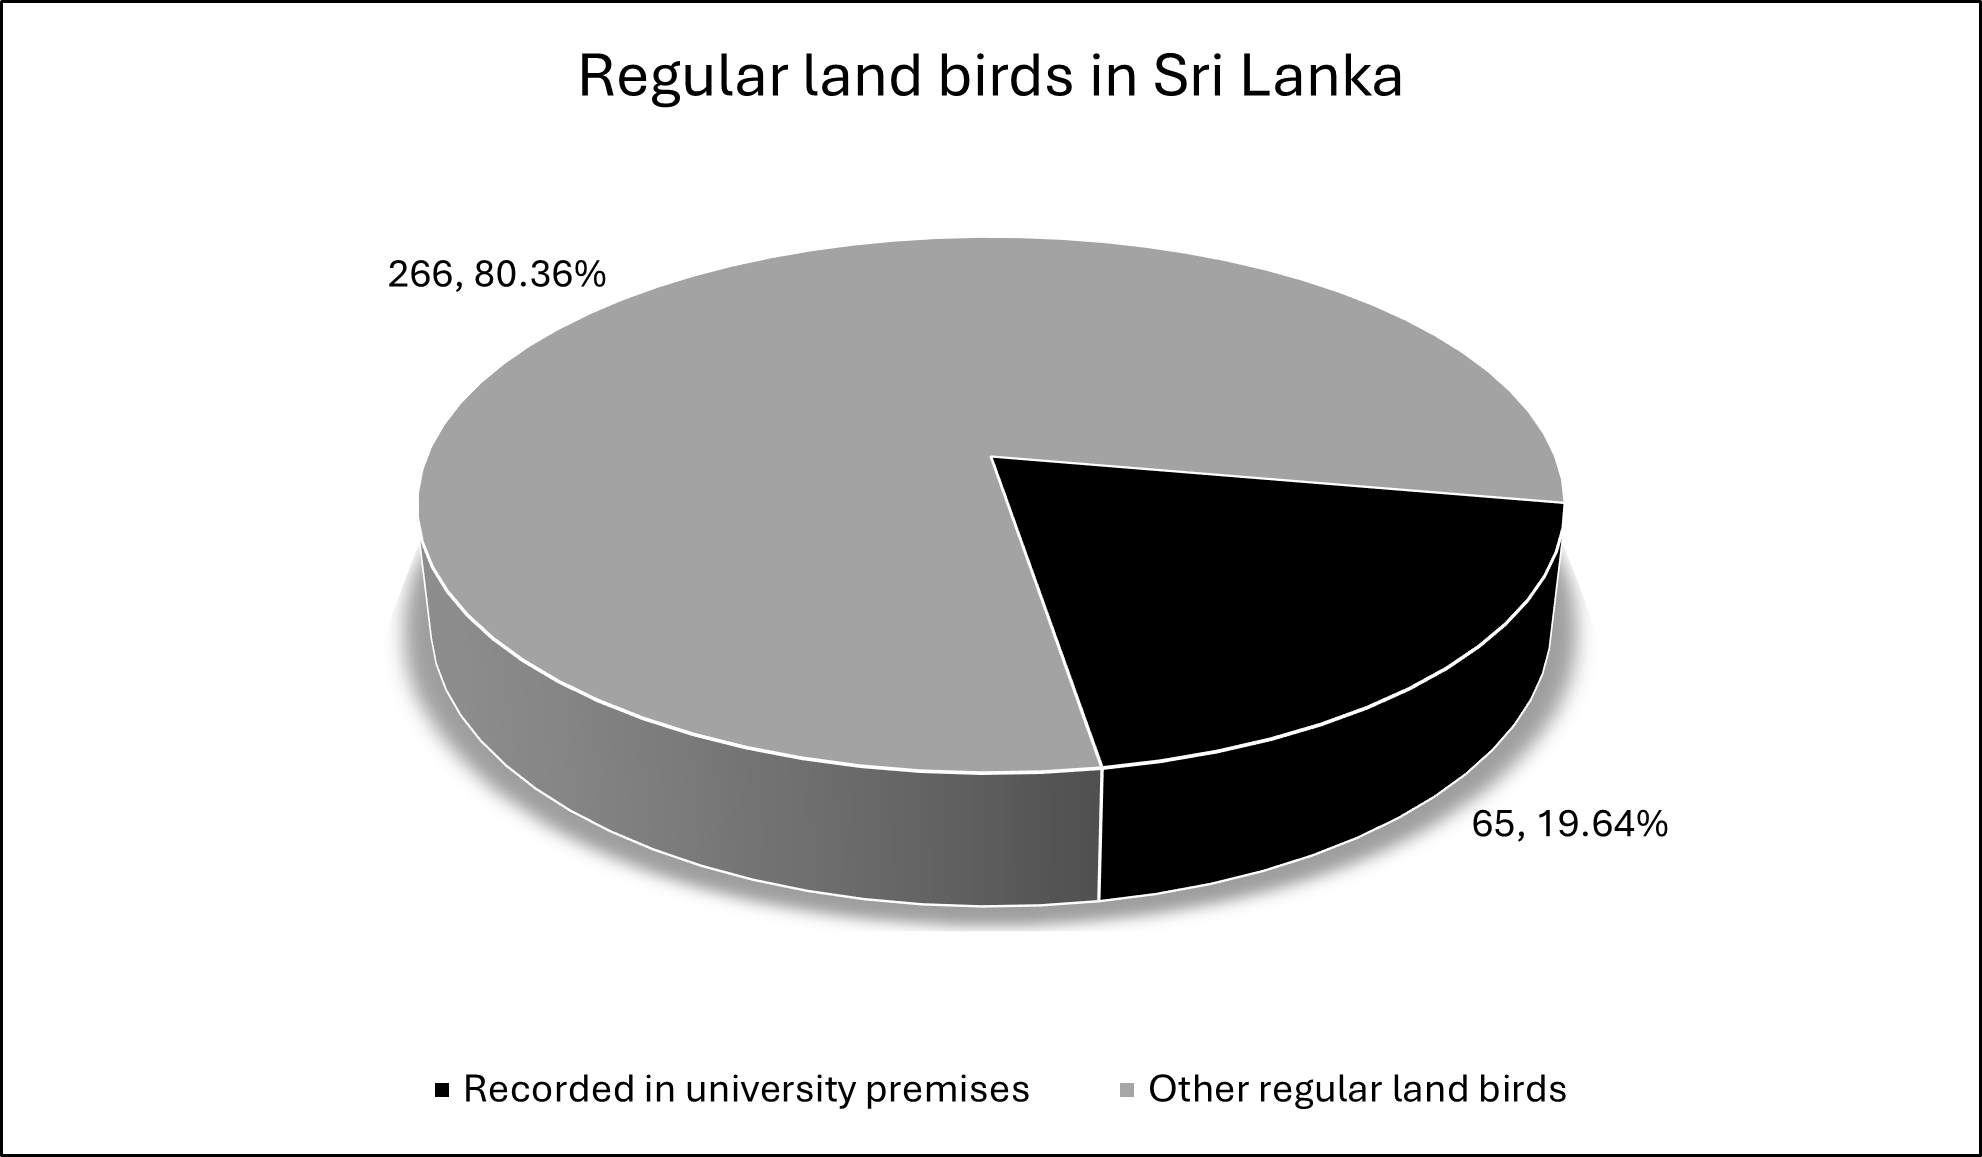
\includegraphics[width=0.9\textwidth]{Figures/pieChart1.png}
    \caption[]{Pie chart showing the recorded number of bird species in the university out of the birds recorded in Sri Lanka.}
    \label{fig:figure-01}
\end{figure}
\noindent 12 out of 88 bird species are migrants to the island while the other 76 species are breeding residents. 

\begin{figure}[!htpb]
    \centering
    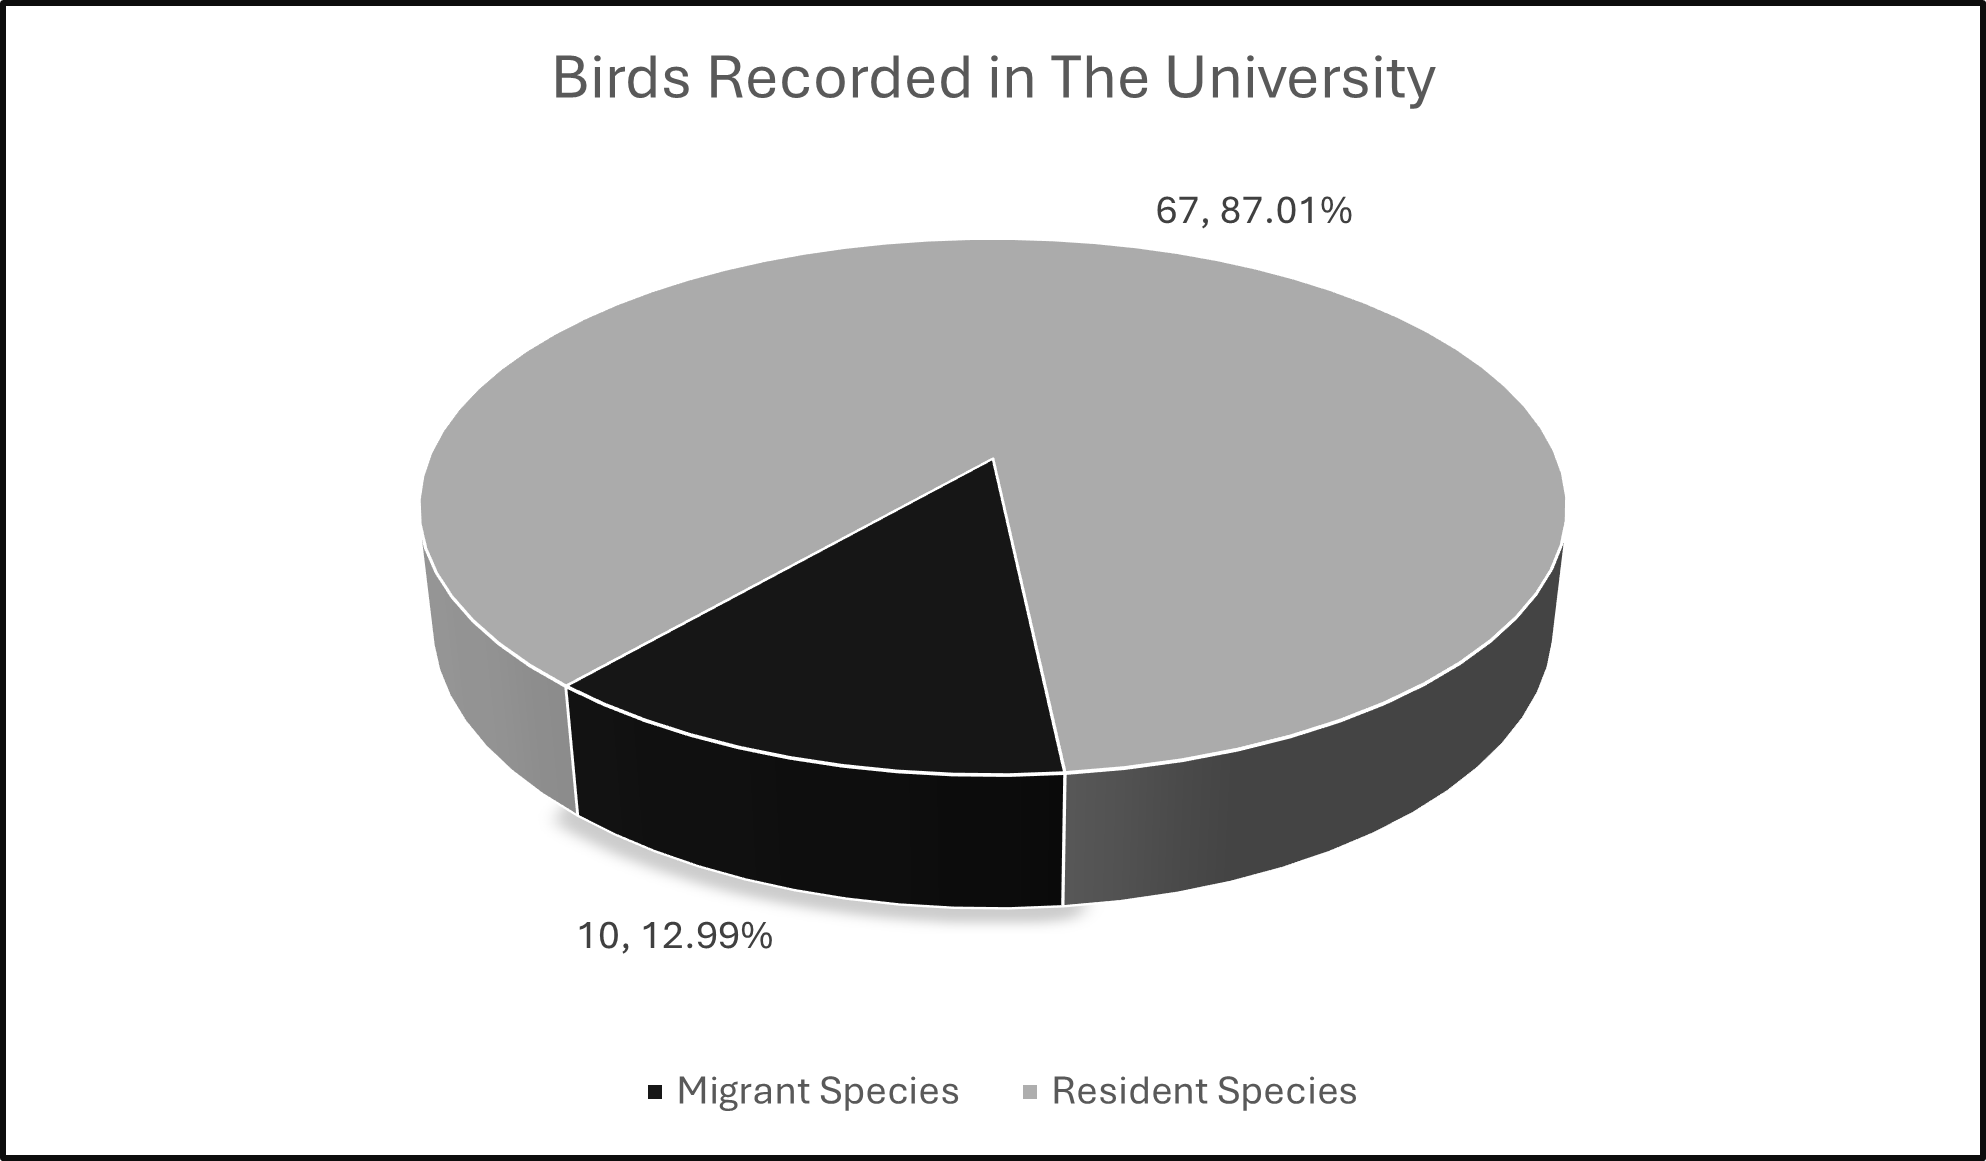
\includegraphics[width=\linewidth]{Figures/pieChart2.png}
    \caption[]{Pie chart showing the number of migrant species and resident species out of total recorded bird species.}
    \label{fig:figure-01}
\end{figure}
\section{Conservation Significance}
The checklist includes single species listed in "Critically Endangered"[3] status, two species listed in "Endangered"[3] status  and another two species listed in "Nearly Threatened"[3] status. 5 out of the recorded 88 birds are endemic to Sri Lanka, including,
\begin{itemize}
\item Crimson-fronted Barbet (\textit{Psilopogon rubricapillus})
\item Red{-}Backed Flameback (\textit{Dinopium psarodes})
\item Sri Lanka Green-Pigeon (\textit{Treron pompadora})
 \item Sri Lanka Hanging-Parrot (\textit{Loriculus beryllinus})
   \item Sri Lanka Swallow (\textit{Cecropis hyperythra})
\end{itemize}
Furthermore, the nests of the following bird species were documented.\footnote{Nests were observed and photographed from a safe distance, utilizing a focal length of at least 650 mm.}
\begin{itemize}
\item Brahminy Kite (\textit{Haliastur indus})
\item Brown-headed Barbet (\textit{Psilopogon zeylanicus})
\item Green Imperial Pigeon (\textit{Ducula aenea})
\item Lesser Whistling{-}Duck (\textit{Dendrocygna javanica})\footnote{Three-four juveniles and a pair of adult specimen seen daily in the Boat yard was the observation.}
\item Purple-rumped Sunbird (\textit{Leptocoma zeylonica})
\item Red-vented Bulbul (\textit{Pycnonotus cafer})
\item Rose-ringed Parakeet (\textit{Psittacula krameri})
\item Scaly-breasted Munia (\textit{Lonchura punctulata})
\item Spotted Dove (\textit{Spilopelia suratensis})
\item Sri Lanka Green-Pigeon (\textit{Treron pompadora})
\item White-bellied Drongo (\textit{Dicrurus caerulescens})
\item White-bellied Sea Eagle (\textit{Haliaeetus leucogaster})
\item White-breasted Waterhen (\textit{Amaurornis phoenicurus})\footnote{Four juveniles and a pair of adult specimen seen daily in the Boat yard was the observation.}
\item White-rumped Munia (\textit{Lonchura striata})
\item Yellow-billed Babbler (\textit{Argya affinis})
\end{itemize}
\vspace*{\fill} %start tag of aligning the image to be bottom of the page.
\begin{figure}[!htpb]
    \centering
    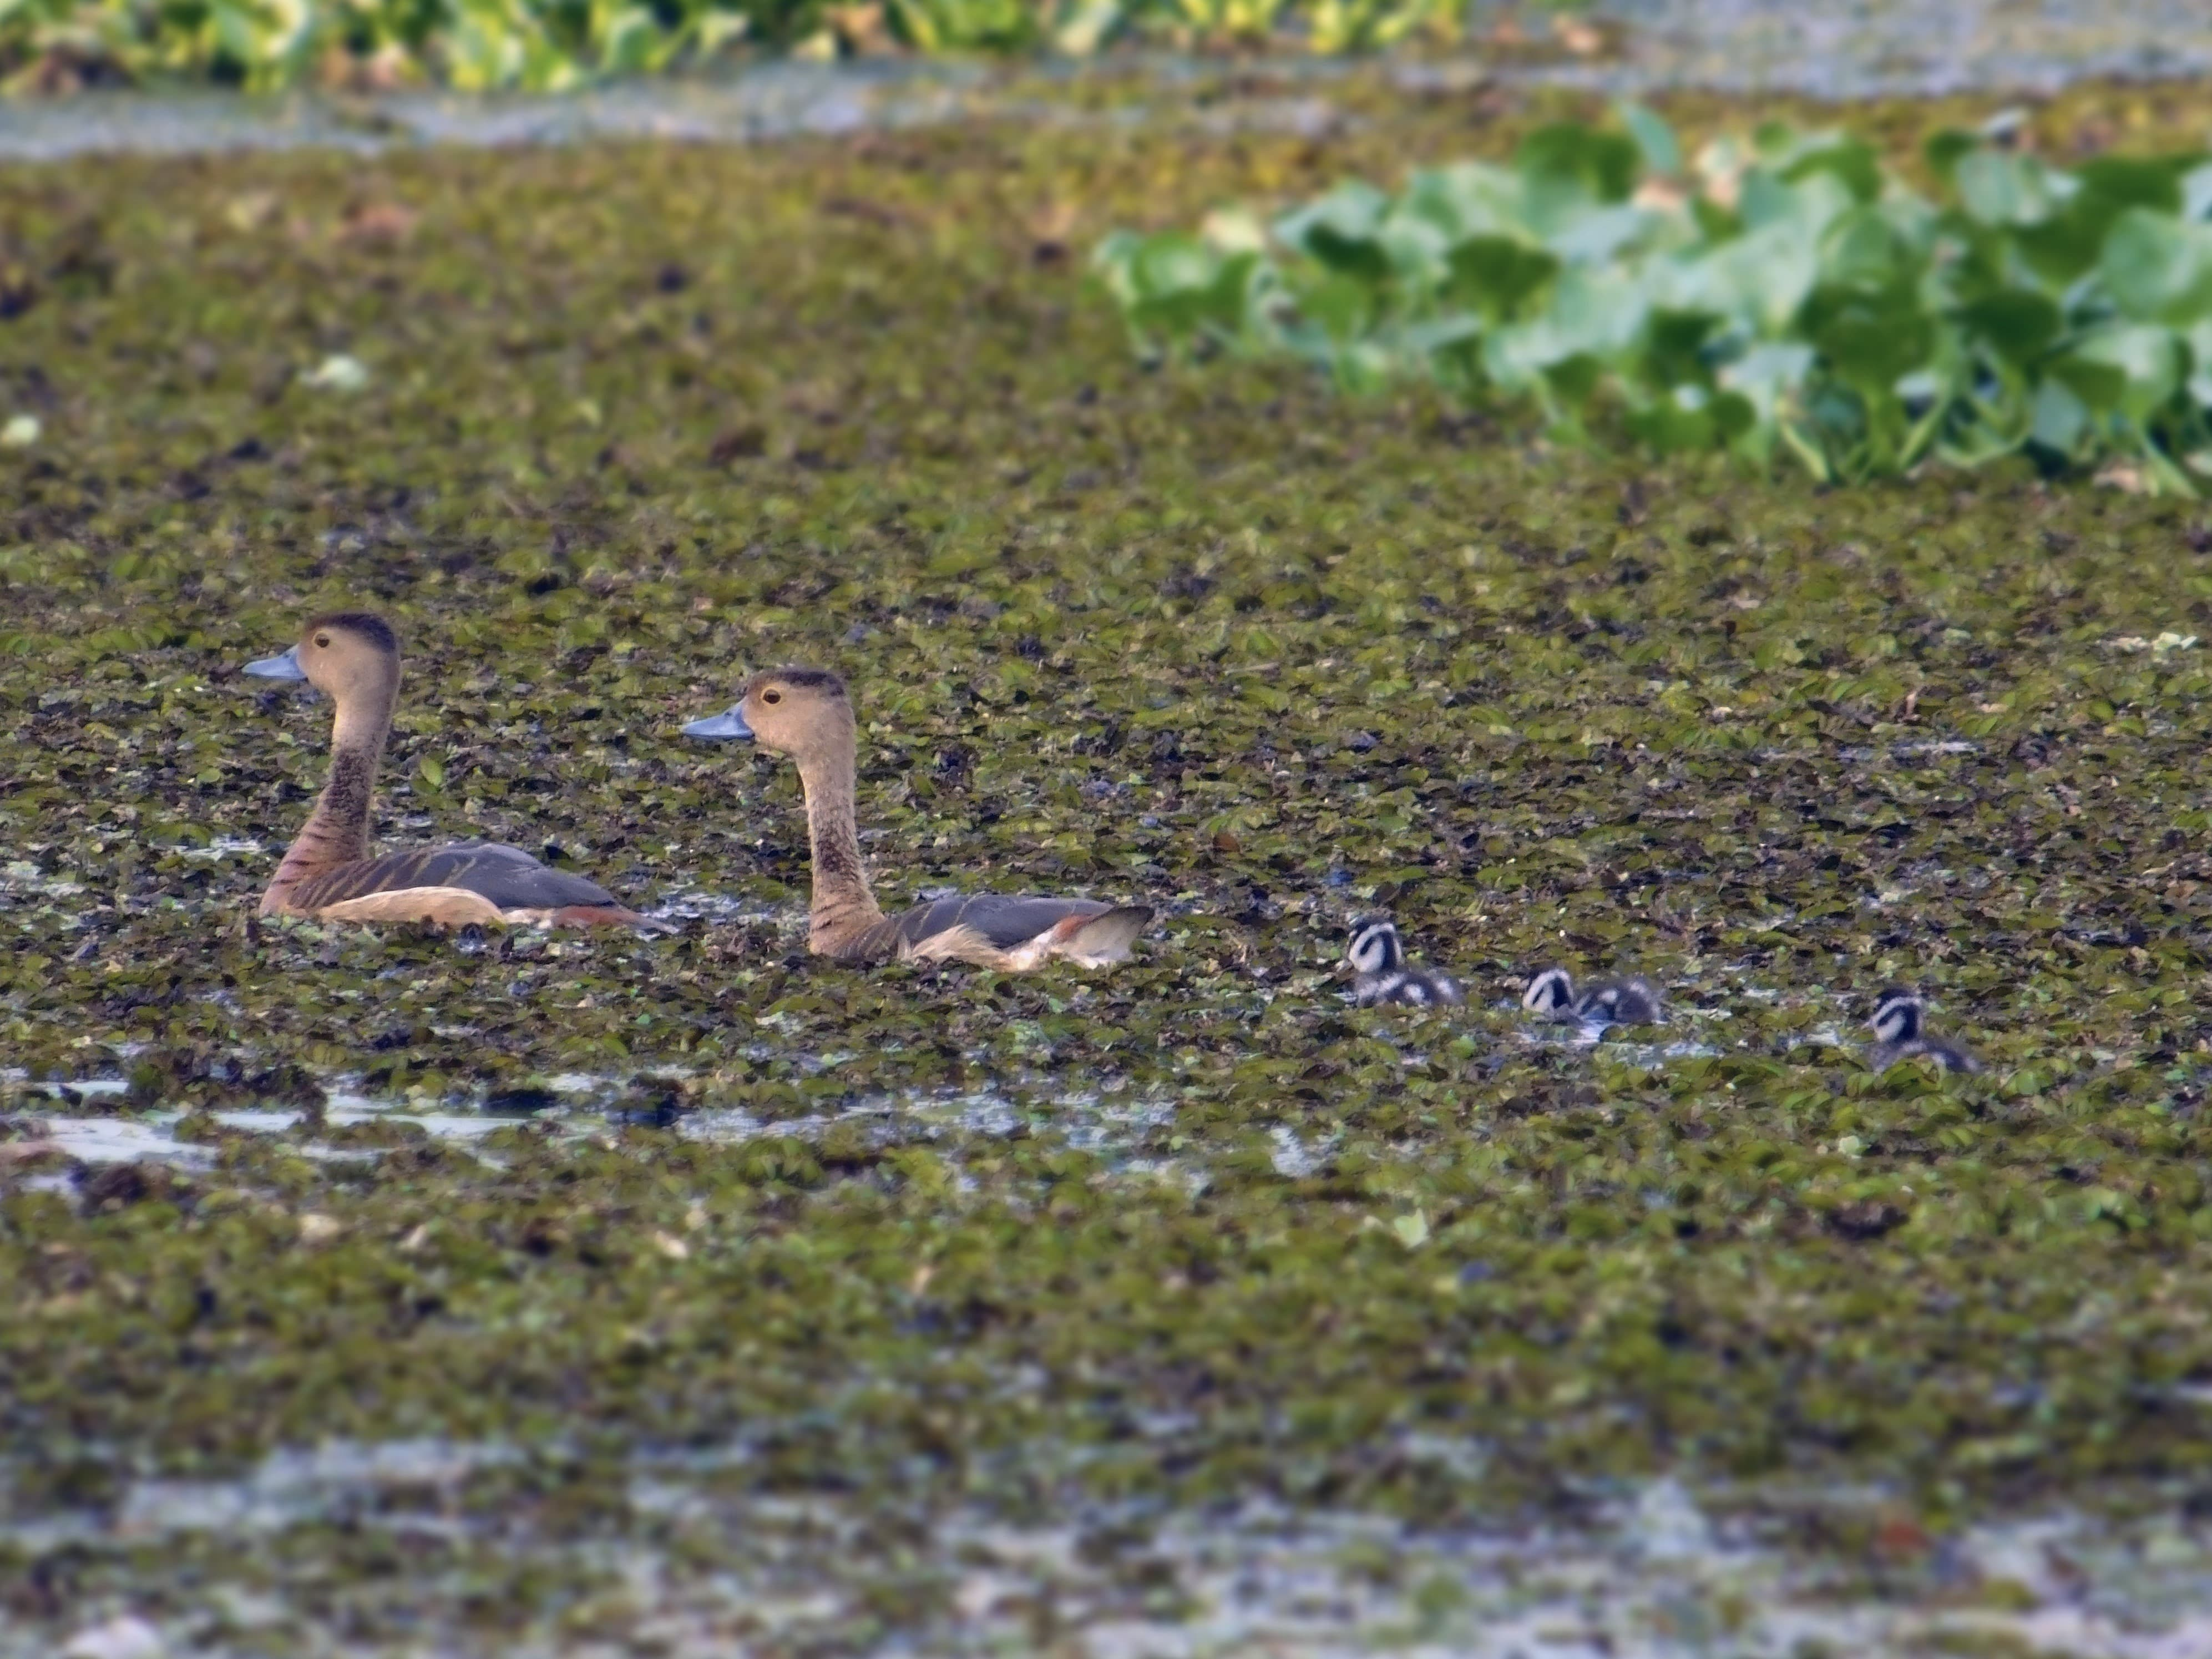
\includegraphics[width=\linewidth]{Figures/whistling-duck.JPG}
    \caption[]{Lesser Whistling{-}Ducks with their offspring, at Boat yard.}
    \label{fig:figure-01}
\end{figure}
\vfill  %end tag of aligning the image to be bottom of the page.
\begin{figure}[!htpb]
    \centering
    \begin{subfigure}{0.45\textwidth}
        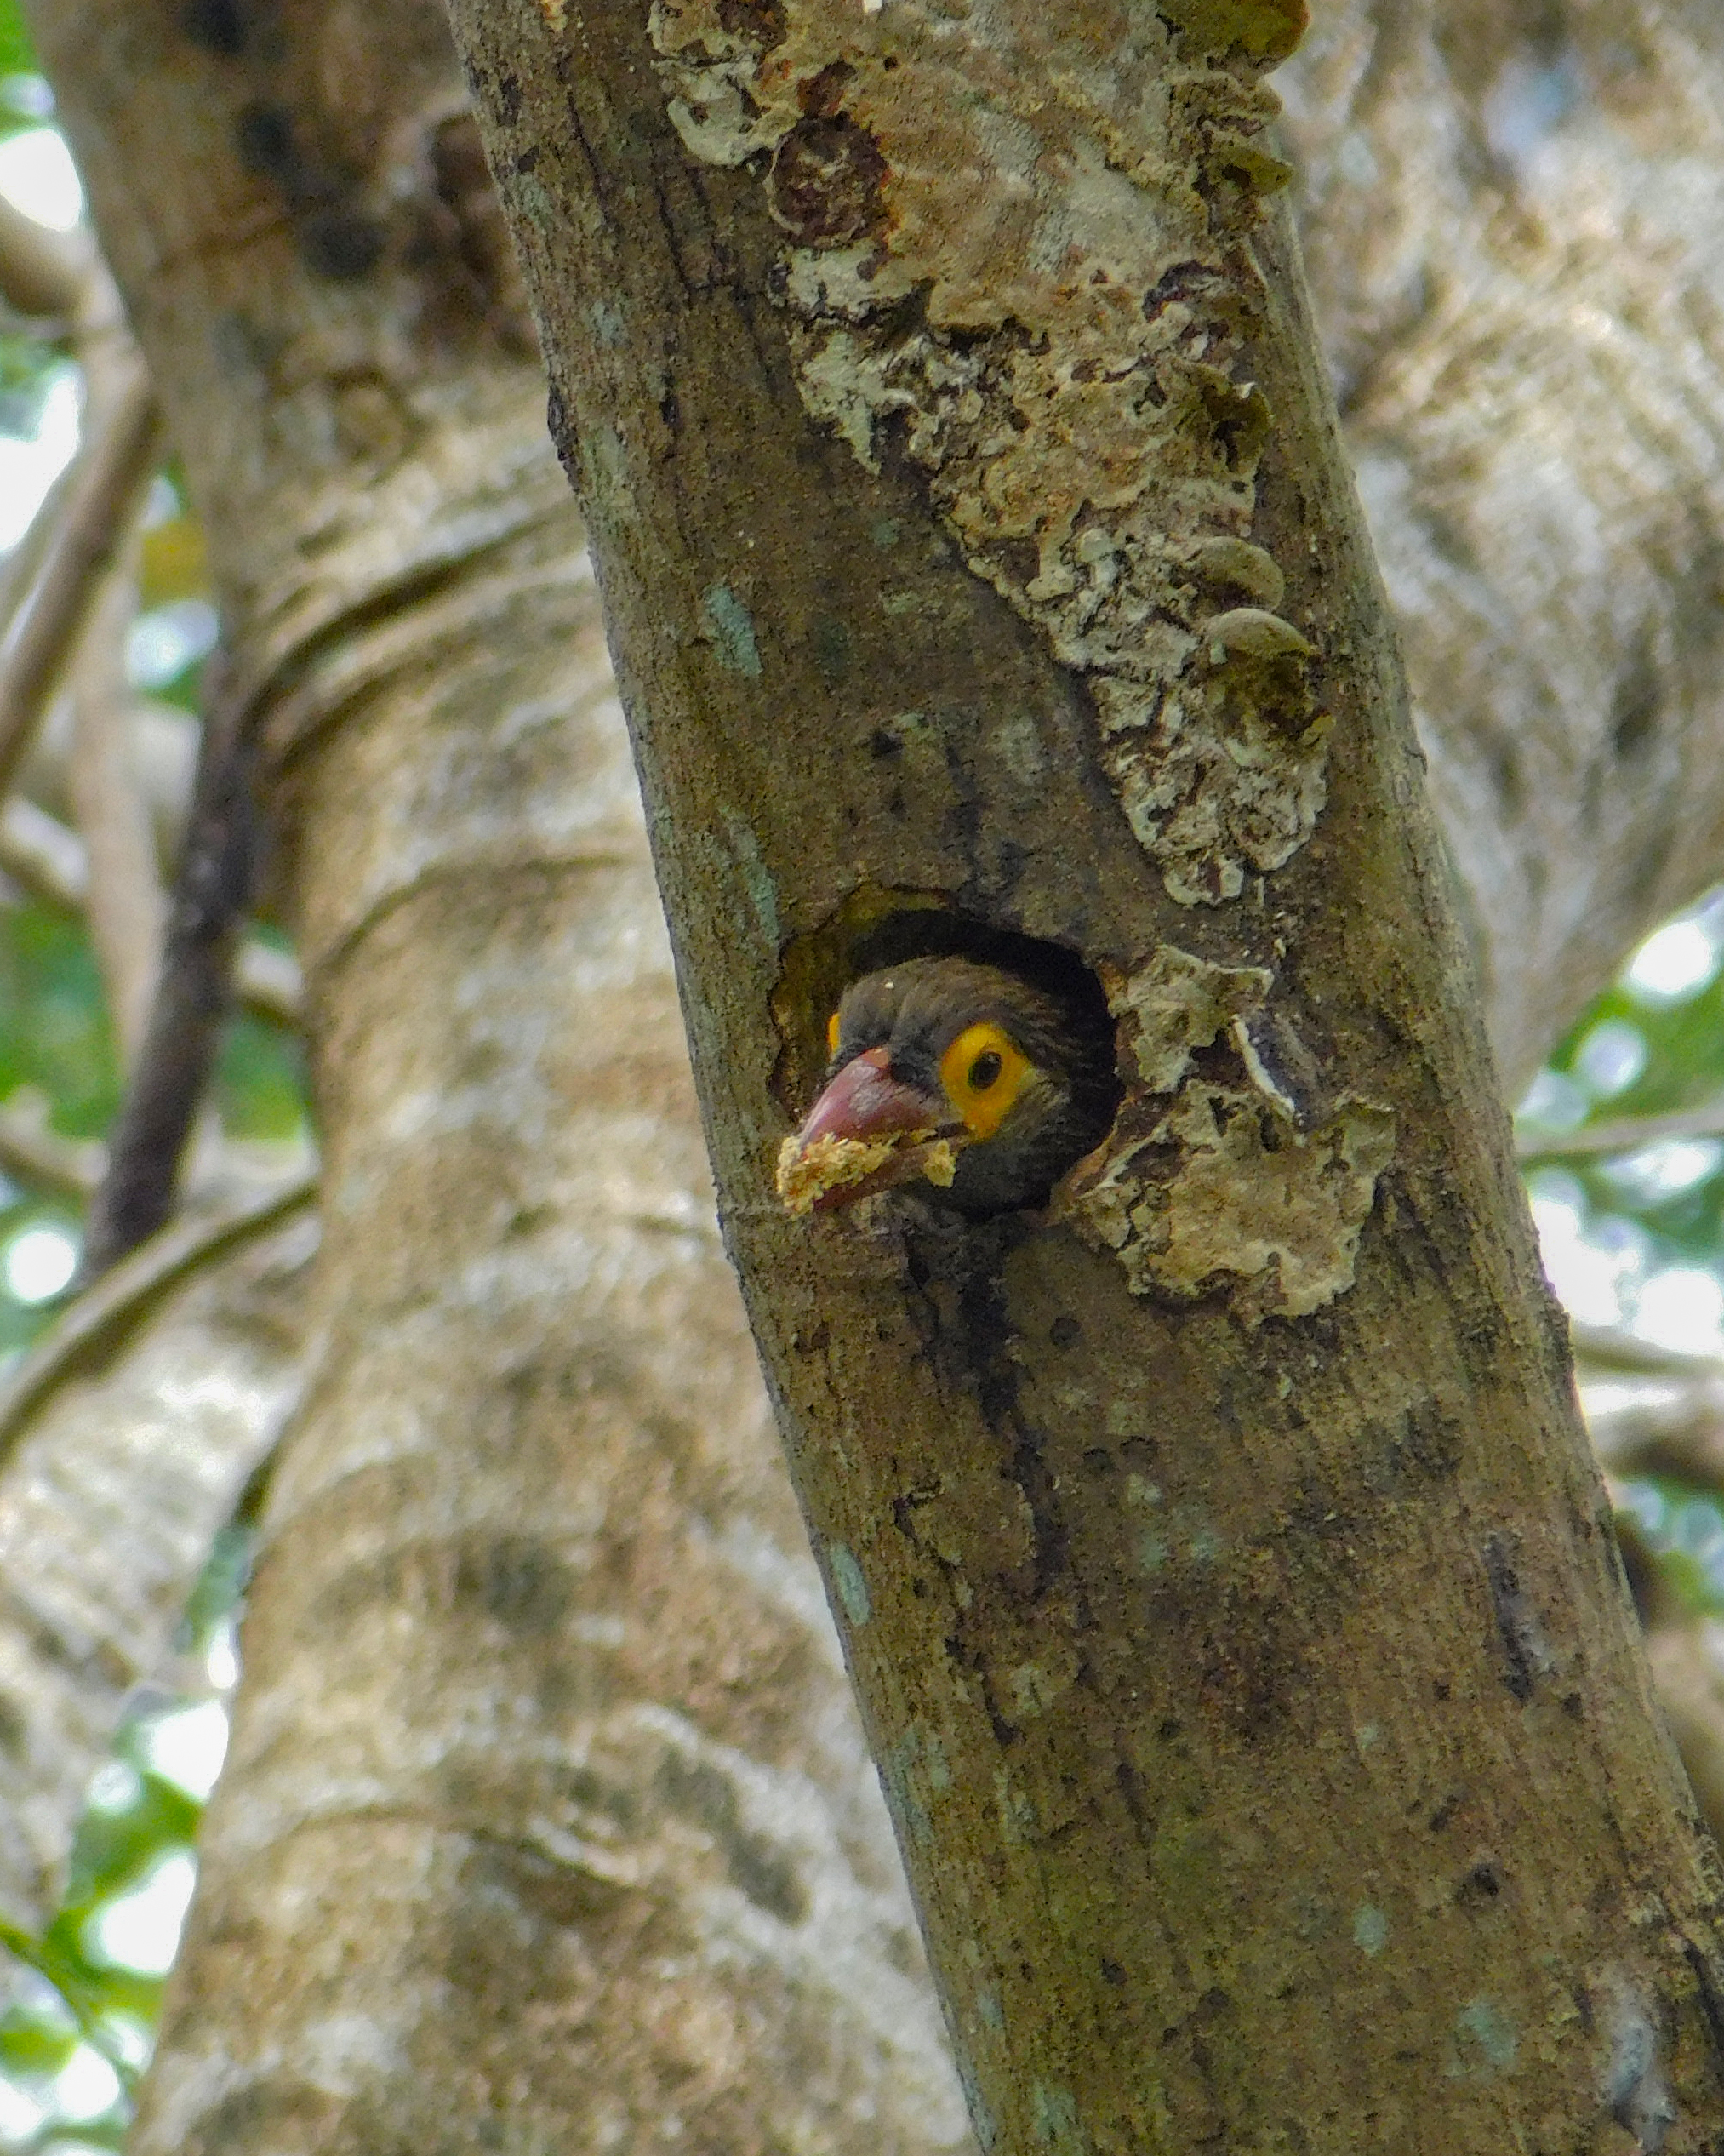
\includegraphics[width=\textwidth]{Figures/brown-headed-barbet.jpg}
        \caption{A Brown-headed Barbet excavating a cavity, Kaju kele.}
        \label{fig:figure-02.1}
    \end{subfigure}
    \hspace{.5cm} % Adjust the space as needed
    \begin{subfigure}{0.45\textwidth}
        \includegraphics[width=\textwidth]{Figures/green-pigeon.jpg}
        \caption{Sri Lanka Green-Pigeon nest near the Dept. of Civil Engineering}
        \label{fig:figure-02.2}
    \end{subfigure}

    
    \begin{subfigure}{0.45\textwidth}
        \includegraphics[width=\textwidth]{Figures/loten's-sun-bird}
        \caption{Purple-rumped Sunbird nest behind the Dept. of Civil Engineering.}
        \label{fig:figure-02.2}
    \end{subfigure}
    \hspace{.5cm} % Adjust the space as needed
    \begin{subfigure}{0.45\textwidth}
        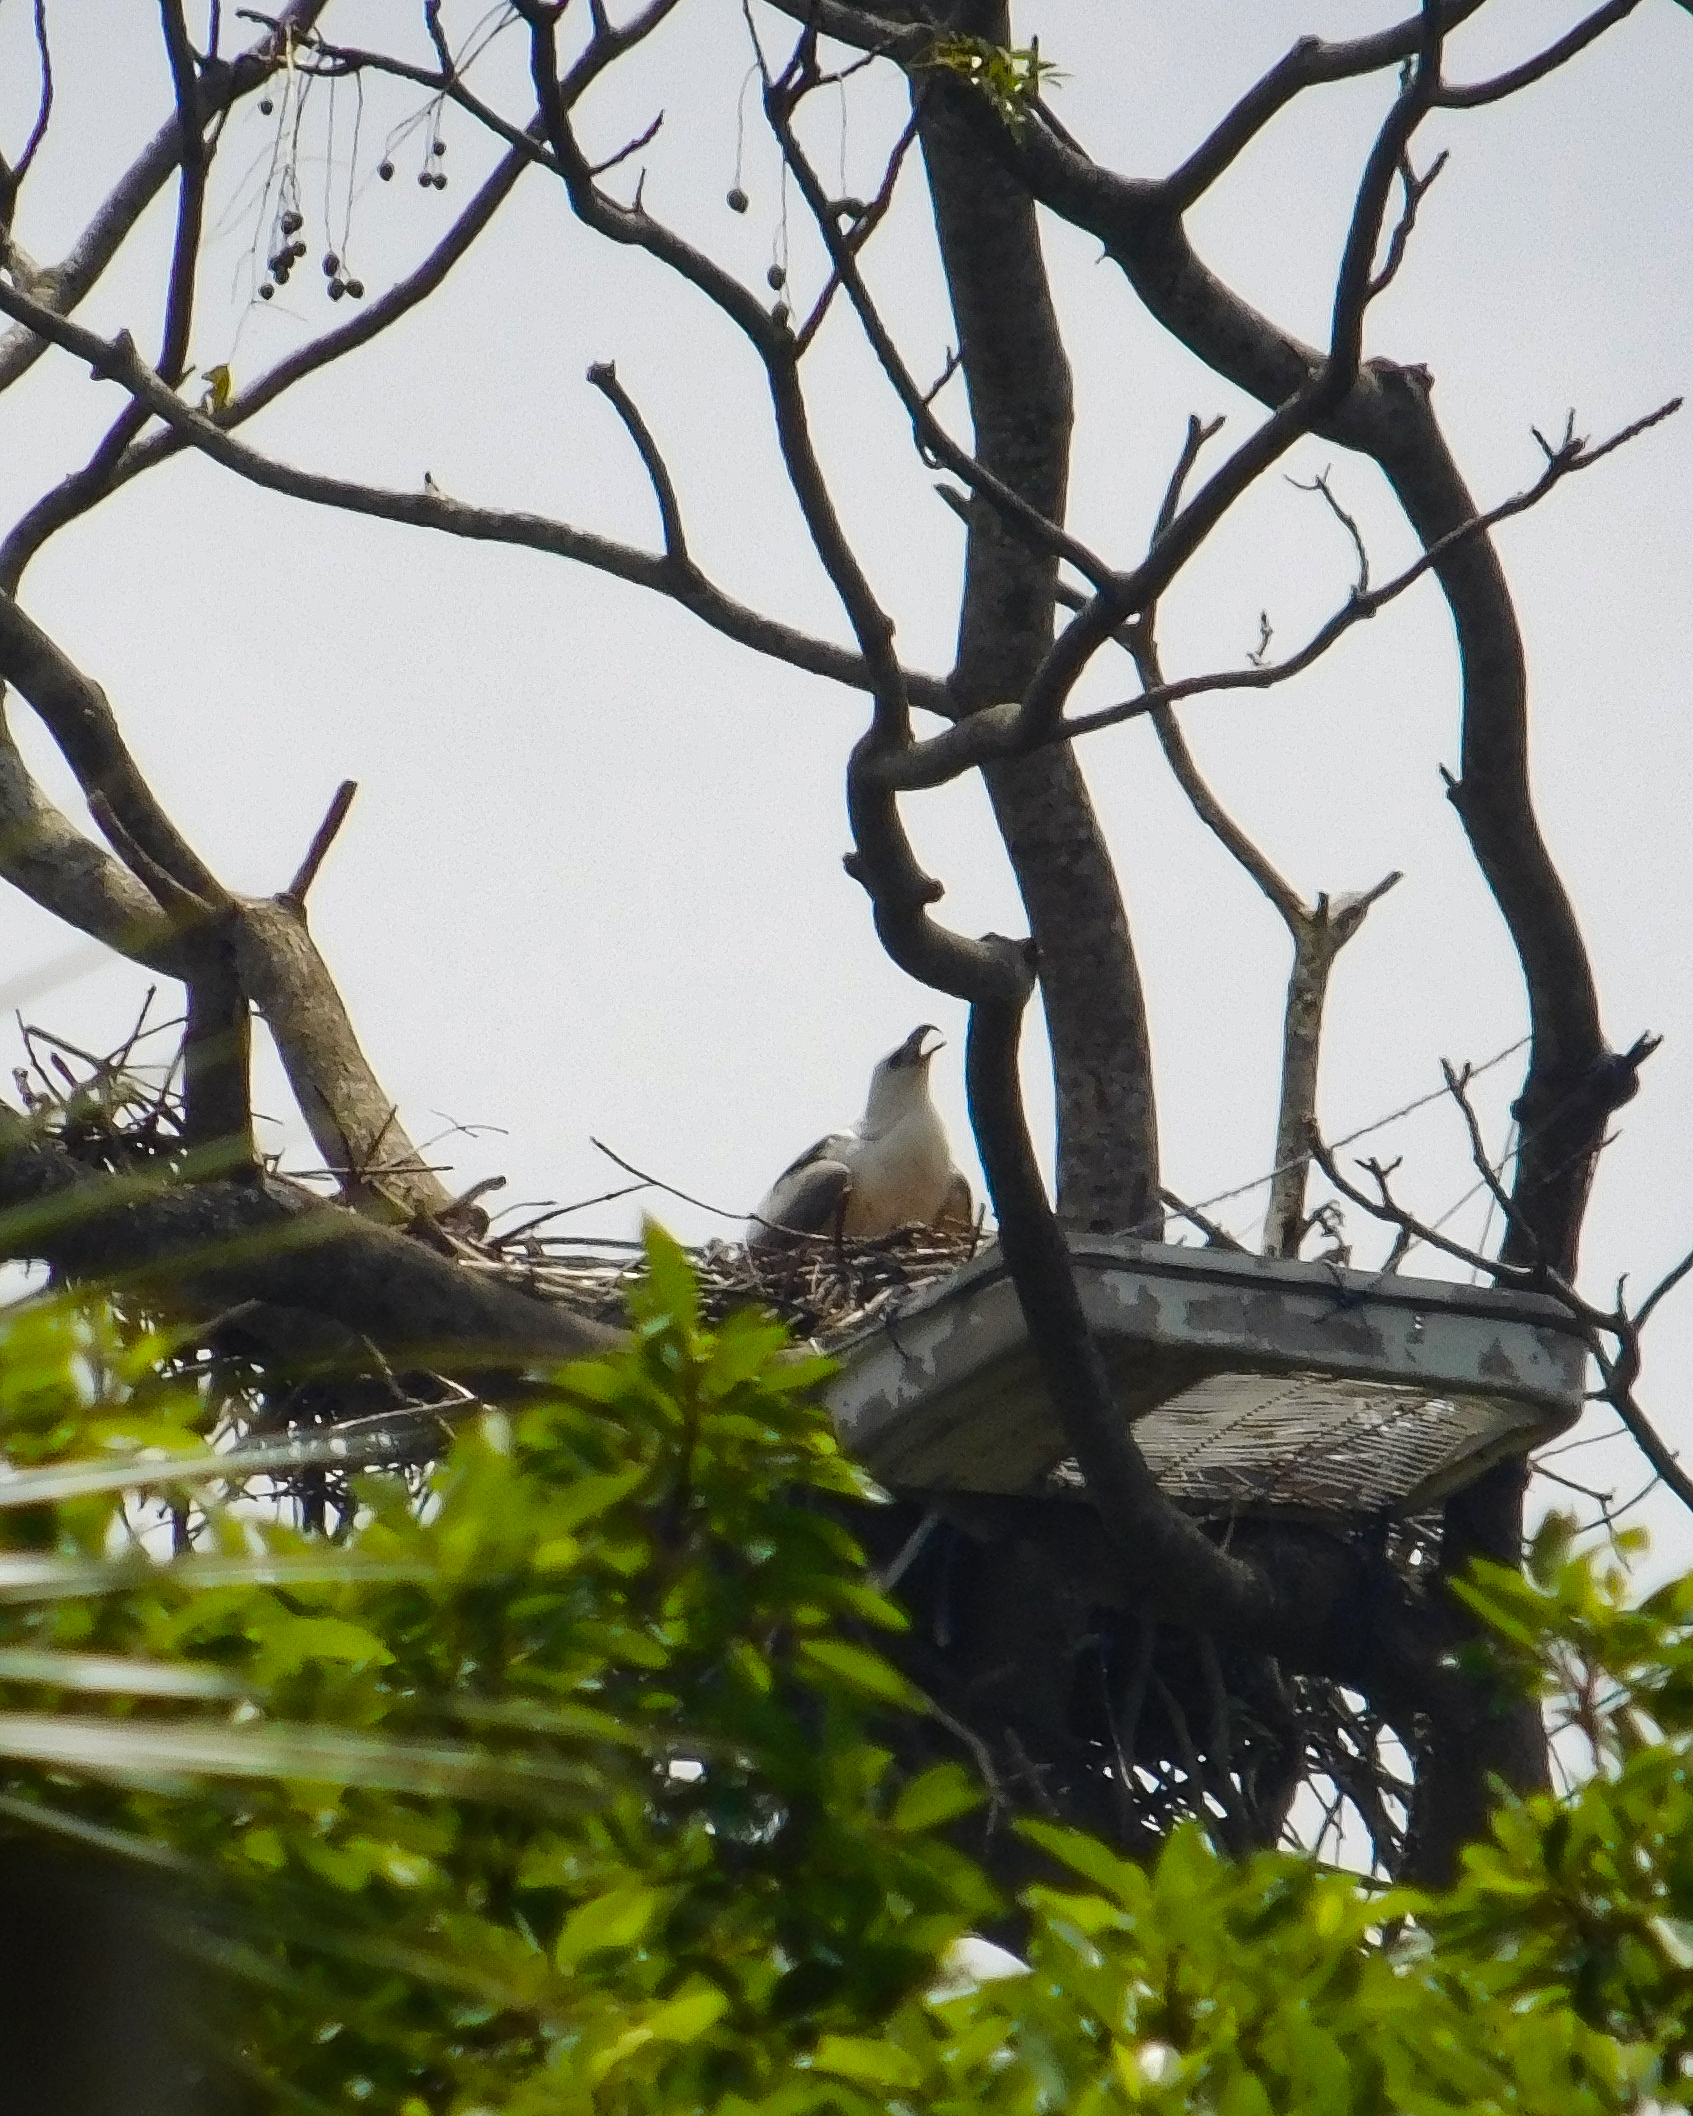
\includegraphics[width=\textwidth]{Figures/white-bellied-sea-eagle.jpg}
        \caption{White-bellied Sea Eagle nest visible to Kaju kele lovers lane.}
        \label{fig:figure-02.2}
    \end{subfigure}
    \caption{Some of the bird nests recorded}
    \label{fig:figure-02}
\end{figure}
% \nameref{cp:citations} (referred to as \autoref{cp:citations}).
\section{Rarity of Species}
While some of the species recorded are very common in the university premises, some others are relatively rare. There were even some species that were recorded only once during the period of study.
\begin{itemize}
    \item Blyth's Reed Warbler (\textit{Acrocephalus dumetorum})
    \item Gray-bellied Cuckoo (\textit{Cacomantis passerinus})
    \item Indian Golden Oriole (\textit{Oriolus kundoo})
    \item Indian Peafowl (\textit{Pavo cristatus})
    \item Indian Robin (\textit{Saxicoloides fulicatus})
    \item Painted Stork (\textit{Mycteria leucocephala})
    \item Black Bittern (\textit{Ixobrychus flavicollis})
\end{itemize}
falls under this category.
\begin{figure}[!htpb]
    \centering
    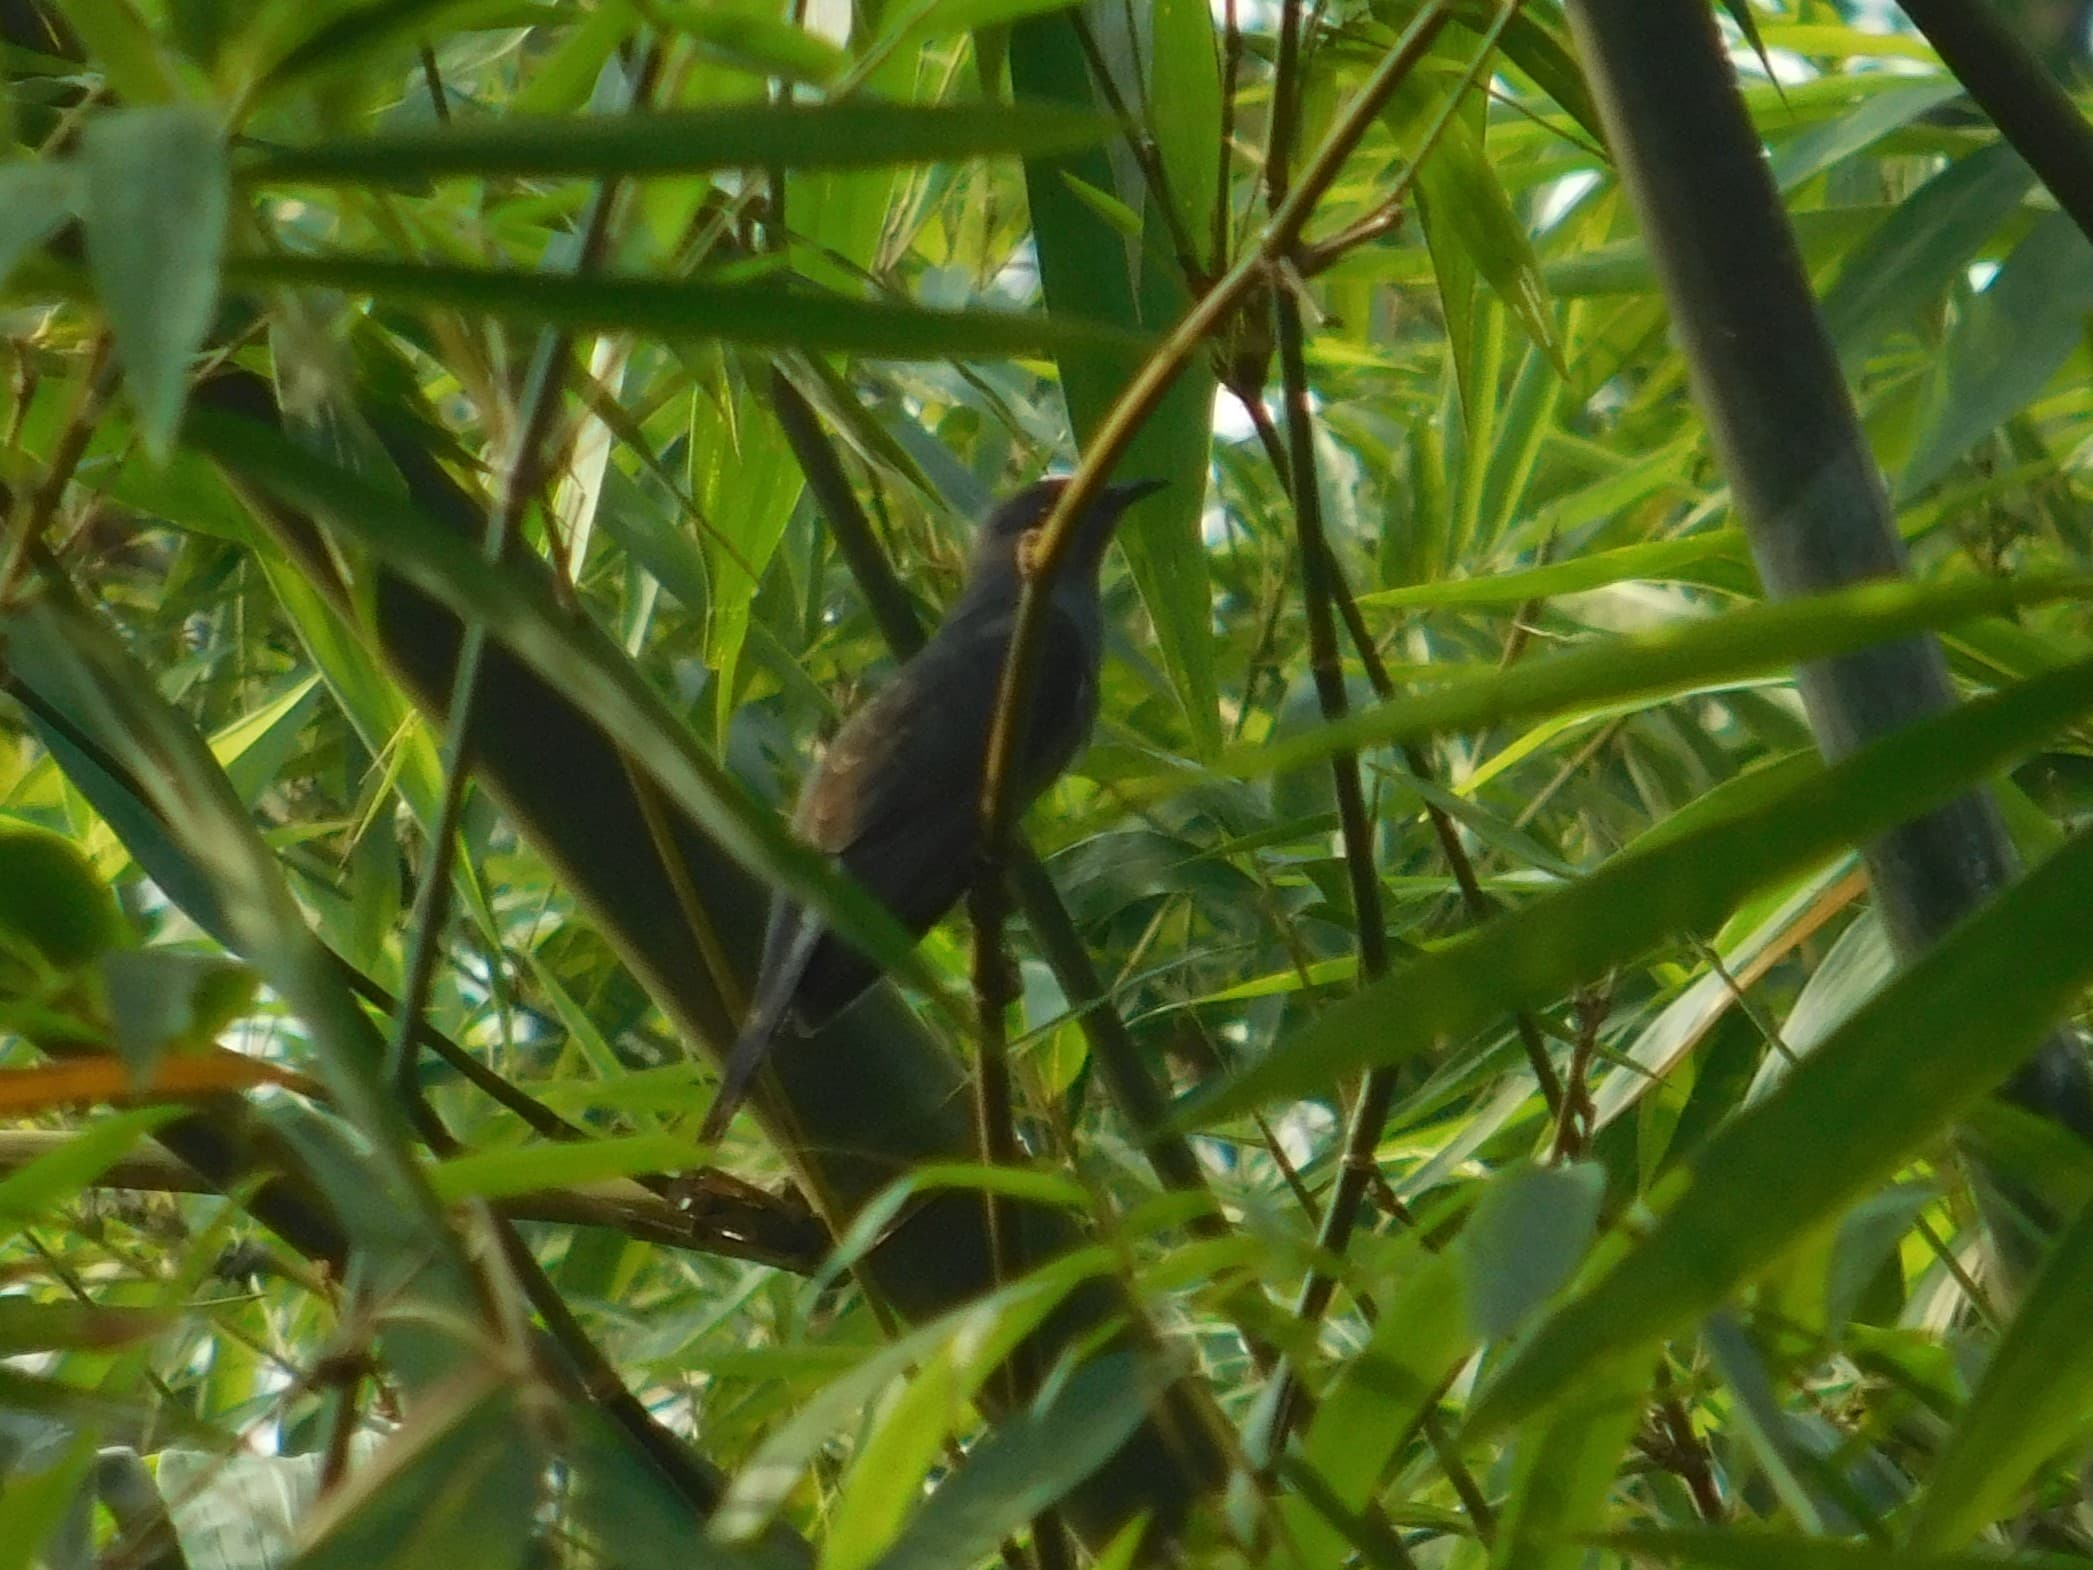
\includegraphics[width=\linewidth]{Figures/gray-bellied-cuckoo.JPG}
    \caption[]{A photograph of the one and only sighting of a Gray-bellied Cuckoo throughout the period of study, taken at "Kaju kele".}
    \label{fig:figure-01}
\end{figure}

